% ============================================================================
% TinyRecursiveControl - Main Figure (Publication-Ready)
% ============================================================================
% Simplified diagram similar to TRM paper figure style
% Compile with: pdflatex paper_figure_main.tex
% ============================================================================

\documentclass[tikz,border=5pt]{standalone}
\usepackage{tikz}
\usepackage{amsmath}
\usetikzlibrary{shapes.geometric, arrows.meta, positioning, calc, fit, backgrounds, decorations.pathreplacing}

% Define colors
\definecolor{inputcolor}{RGB}{66, 133, 244}
\definecolor{encodercolor}{RGB}{52, 168, 83}
\definecolor{reasoningcolor}{RGB}{251, 188, 4}
\definecolor{decodercolor}{RGB}{234, 67, 53}
\definecolor{outputcolor}{RGB}{156, 39, 176}
\definecolor{feedbackcolor}{RGB}{255, 87, 34}
\definecolor{latentcolor}{RGB}{0, 150, 136}
\definecolor{loopcolor}{RGB}{100, 100, 100}

\begin{document}

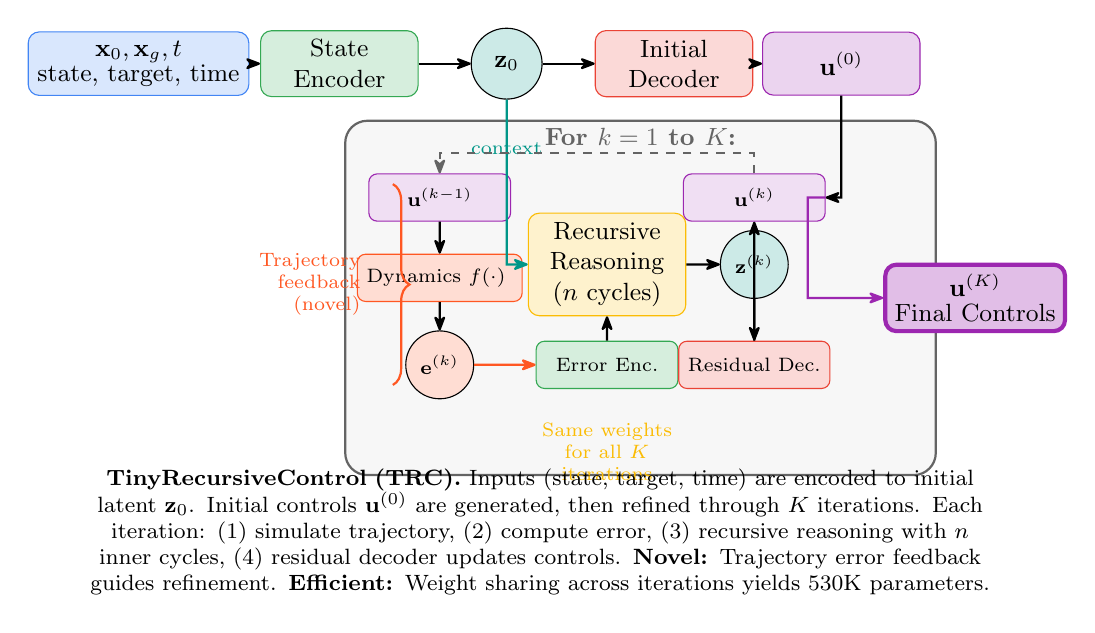
\begin{tikzpicture}[
    scale=0.85,
    node distance=1cm,
    >={Stealth[round]},
    box/.style={rectangle, rounded corners=4pt, draw, minimum width=2cm, minimum height=0.8cm, align=center, font=\small},
    smallbox/.style={rectangle, rounded corners=3pt, draw, minimum width=1.8cm, minimum height=0.6cm, align=center, font=\scriptsize},
    latent/.style={circle, draw, fill=#1!20, minimum size=0.9cm, font=\small},
    arrow/.style={->, thick},
    label/.style={font=\footnotesize},
    tinylabel/.style={font=\scriptsize}
]

% =================== TOP: TRC Flow ===================

% Inputs (stacked)
\node[box, fill=inputcolor!20, draw=inputcolor] (inputs) at (0, 0) {
    $\mathbf{x}_0, \mathbf{x}_g, t$\\[-2pt]
    \tinylabel{state, target, time}
};

% State Encoder
\node[box, fill=encodercolor!20, draw=encodercolor] (encoder) at (3, 0) {
    State\\Encoder
};

% Initial latent z0
\node[latent=latentcolor] (z0) at (5.5, 0) {$\mathbf{z}_0$};

% Initial decoder
\node[box, fill=decodercolor!20, draw=decodercolor] (init_dec) at (8, 0) {
    Initial\\Decoder
};

% Initial controls
\node[box, fill=outputcolor!20, draw=outputcolor] (u0) at (10.5, 0) {$\mathbf{u}^{(0)}$};

% Arrows for initial path
\draw[arrow] (inputs) -- (encoder);
\draw[arrow] (encoder) -- (z0);
\draw[arrow] (z0) -- (init_dec);
\draw[arrow] (init_dec) -- (u0);

% =================== REFINEMENT LOOP ===================

% Loop box background
\begin{scope}[on background layer]
\node[draw=loopcolor, thick, rounded corners=8pt, fill=loopcolor!5,
      minimum width=7.5cm, minimum height=4.5cm] (loopbox) at (7.5, -3.5) {};
\end{scope}

% Loop label
\node[font=\small\bfseries, text=loopcolor] at (7.5, -1.1) {
    For $k = 1$ to $K$:
};

% Inside loop - Current controls input
\node[smallbox, fill=outputcolor!15, draw=outputcolor] (uk_in) at (4.5, -2) {$\mathbf{u}^{(k-1)}$};

% Dynamics simulation
\node[smallbox, fill=feedbackcolor!20, draw=feedbackcolor] (sim) at (4.5, -3.2) {
    Dynamics $f(\cdot)$
};

% Error
\node[latent=feedbackcolor, minimum size=0.7cm] (error) at (4.5, -4.5) {\scriptsize$\mathbf{e}^{(k)}$};

% Error encoder
\node[smallbox, fill=encodercolor!20, draw=encodercolor] (err_enc) at (7, -4.5) {Error Enc.};

% Reasoning block (main)
\node[box, fill=reasoningcolor!20, draw=reasoningcolor, minimum height=1.2cm] (reason) at (7, -3) {
    Recursive\\Reasoning\\($n$ cycles)
};

% z0 injection arrow
\draw[arrow, latentcolor] (z0) -- (5.5, -3) -- (reason.west);
\node[tinylabel, text=latentcolor, anchor=south] at (5.5, -1.5) {context};

% Updated latent
\node[latent=latentcolor, minimum size=0.7cm] (zk) at (9.2, -3) {\scriptsize$\mathbf{z}^{(k)}$};

% Residual decoder
\node[smallbox, fill=decodercolor!20, draw=decodercolor] (res_dec) at (9.2, -4.5) {Residual Dec.};

% Updated controls
\node[smallbox, fill=outputcolor!15, draw=outputcolor] (uk_out) at (9.2, -2) {$\mathbf{u}^{(k)}$};

% Arrows inside loop
\draw[arrow] (uk_in) -- (sim);
\draw[arrow] (sim) -- (error);
\draw[arrow, feedbackcolor] (error) -- (err_enc);
\draw[arrow] (err_enc) -- (reason);
\draw[arrow] (reason) -- (zk);
\draw[arrow] (zk) -- (res_dec);
\draw[arrow] (res_dec) -- (uk_out);

% Loop back arrow
\draw[arrow, loopcolor, dashed] (uk_out.north) -- ++(0, 0.3) -- ($(uk_in.north) + (0, 0.3)$) -- (uk_in.north);

% =================== FINAL OUTPUT ===================

% Arrow from u0 to loop
\draw[arrow] (u0) -- (10.5, -2) -- (uk_out);

% Final output
\node[box, fill=outputcolor!30, draw=outputcolor, line width=1.5pt] (final) at (12.5, -3.5) {
    $\mathbf{u}^{(K)}$\\[-2pt]
    \tinylabel{Final Controls}
};

\draw[arrow, outputcolor, thick] (uk_out) -- ++(0.8, 0) |- (final);

% =================== ANNOTATIONS ===================

% Key mechanism highlight
\draw[decorate, decoration={brace, amplitude=6pt, mirror}, feedbackcolor, thick]
    (3.8, -4.8) -- (3.8, -1.8) node[midway, left=8pt, font=\scriptsize, text=feedbackcolor, align=right] {
        Trajectory\\feedback\\(novel)
    };

% Weight sharing annotation
\node[tinylabel, text=reasoningcolor, text width=2cm, align=center] at (7, -5.8) {
    Same weights\\for all $K$ iterations
};

% =================== CAPTION ===================
\node[font=\footnotesize, text width=12cm, align=center] at (6, -7) {
    \textbf{TinyRecursiveControl (TRC).}
    Inputs (state, target, time) are encoded to initial latent $\mathbf{z}_0$.
    Initial controls $\mathbf{u}^{(0)}$ are generated, then refined through $K$ iterations.
    Each iteration: (1) simulate trajectory, (2) compute error, (3) recursive reasoning with $n$ inner cycles,
    (4) residual decoder updates controls.
    \textbf{Novel:} Trajectory error feedback guides refinement.
    \textbf{Efficient:} Weight sharing across iterations yields 530K parameters.
};

\end{tikzpicture}

\end{document}
